

\chapter{Product Evaluation and AI Assistant in VitamiNurse}
\section*{Introduction}
\addcontentsline{toc}{section}{Introduction}
The VitamiNurse app stands out from other traditional nutrition apps through its advanced use of artificial intelligence .

In addition to the use of a sentence transformer model to generate vector embeddings in the recommendation system discussed earlier, this section introduces two key AI components: a product evaluation system and an AI assistant.

This integration of AI transforms static product recommendations into an interactive dialogue system that is available 24/7 to answer questions and provide nutritional guidance. The following sections detail the architecture and functionality of these AI systems within the VitamiNurse mobile app.

\section{Advanced scan system with AI analysis }

Instead of showing large amounts of raw product data, it uses AI to interpret the product after scanning its barcode.  Through the combination of detailed nutritional information, user health profiles, and AI reasoning based on prompts, the VitamiNurse app provides customized nutritional guidance in a way that traditional tools cannot. The result is a highly interactive and user-friendly experience that transforms a simple scan into an informed decision-making process.

\subsection{Prompt Engineering for AI Analysis}
\par In addition to the details of the product that appear on the screen after scanning the barcode, we added an AI analytics system to provide a concise and personalized conclusion.
 The generative AI capabilities of our system are powered by a popular pre-trained LLM, which is ChatGPT-4, to build accurate and relevant responses.
 \par The system uses structured prompts to guide AI during product evaluation.
The following code illustrates how each prompt integrates essential product information with user-specific data, including health conditions and allergies, to determine the suitability of the product for the user profile.
\begin{center}
\begin{figure}[H]
    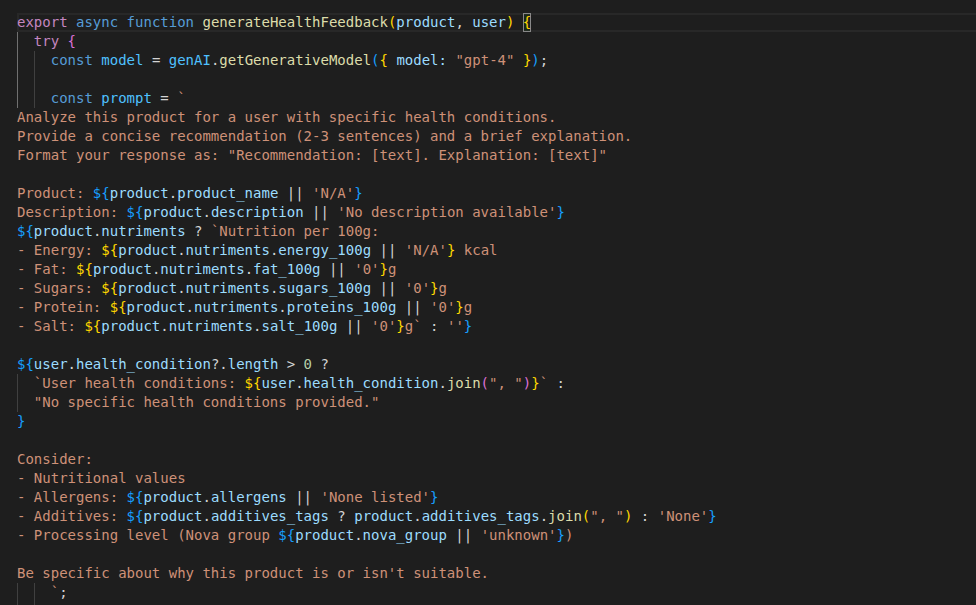
\includegraphics[width=0.9\textwidth]{images/prompt_engineering.png}
    \caption{Prompt Engineering Using GPT-4} 
    \label{fig:Prompt_Engineering}
\end{figure}
\end{center}

\subsection{System Operation in VitamiNurse}
The AI analysis system in VitamiNurse integrates a product scanning feature with real-time health feedback, powered by a combination of external APIs, a MongoDB database, and the ChatGPT-4 model. Users can scan a barcode (EAN) to retrieve detailed nutritional information, which is cross-referenced with their health profile stored in the users collection. The system first checks our database for existing product data. If it is unavailable, it fetches data from the OpenFoodFacts API and caches it for future use. The AI then processes these data alongside user health conditions to generate personalized feedback: \textbf{Is this product suitable or not, and why?}
The following picture illustrates how the user see the details of the scanned product and generated health feedback by the AI analytics system:
\begin{center}
    \begin{figure}[H]
    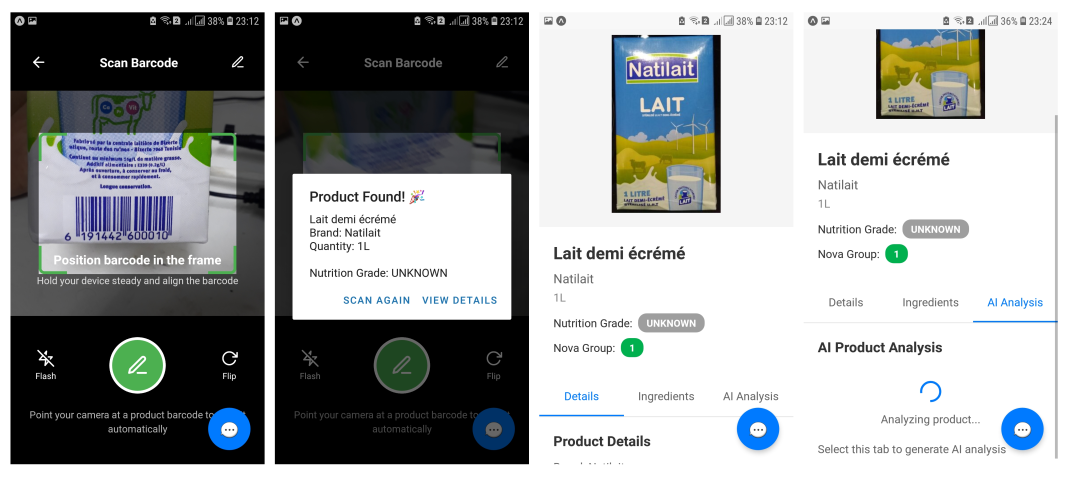
\includegraphics[width=0.9\textwidth]{images/natilait.png}
    \caption{Product evaluation and AI analysis in VitamiNurse app}
    \label{fig:main_figure}
\end{figure}
\end{center}

\section{The AI Assistant}
The AI nutrition assistant represents a new generation of personalized dietary advice and nutritional data analysis, all within a coherent conversational interface.
\section{System Architecture}
The architecture of the Nutrition Assistant is designed for modularity, scalability, and maintainability. Figure~\ref{fig:chatbot_Architect_layers} outlines this three-tier architecture, consisting of the user mobile interface, backend server, and AI/data layer.
 This separation ensures that improvements in one layer, such as up-grading the recommendation logic, can be implemented without disrupting other components of the system. The conversational capabilities of this intuitive chatbot are tightly integrated with a persistent memory framework in order to recall previous user interactions and adapt recommendations over time.  
\begin{figure}[H]
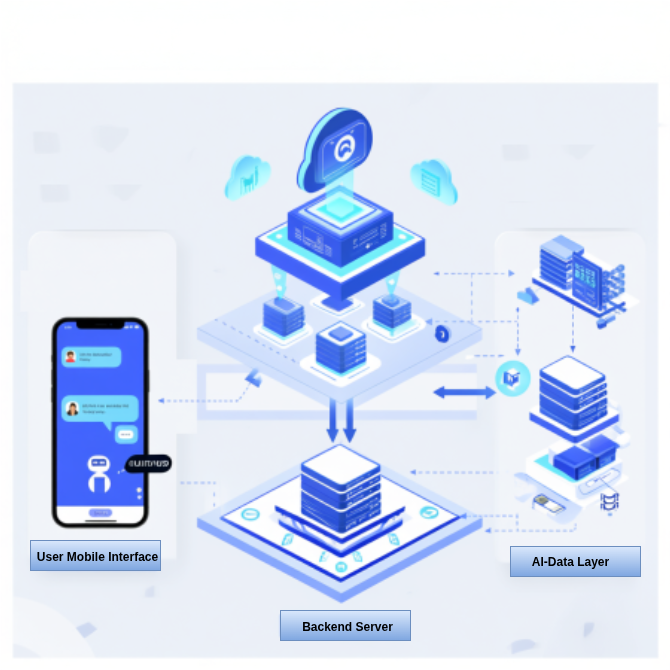
\includegraphics[width=0.9\textwidth]{images/chat_layers.png}
\caption{Chatbot Architecture} 
\label{fig:chatbot_Architect_layers}
\end{figure}

\subsection{User Mobile Interface}
The mobile interface functions as the central interaction point for users
engaging with the VitamiNurse assistant, supporting key features such
as conversational dialogue and product scanning. When a user scans a
product barcode or types a question, the interface sends a structured
request to the backend, which in turn invokes the AI modules for analysis.
The design emphasizes simplicity and readability, ensuring that even
complex nutritional assessments are communicated in concise and easy-to-understand language. 
This is achieved through the adoption of a fixed
“Recommendation + Explanation” format, which the AI adheres to
when generating responses. The application returns the scanned product’s details and nutritional breakdowns as well as AI analysis for this product,
making the experience both informative and engaging.

\begin{center}
\begin{figure}[H]
\centering
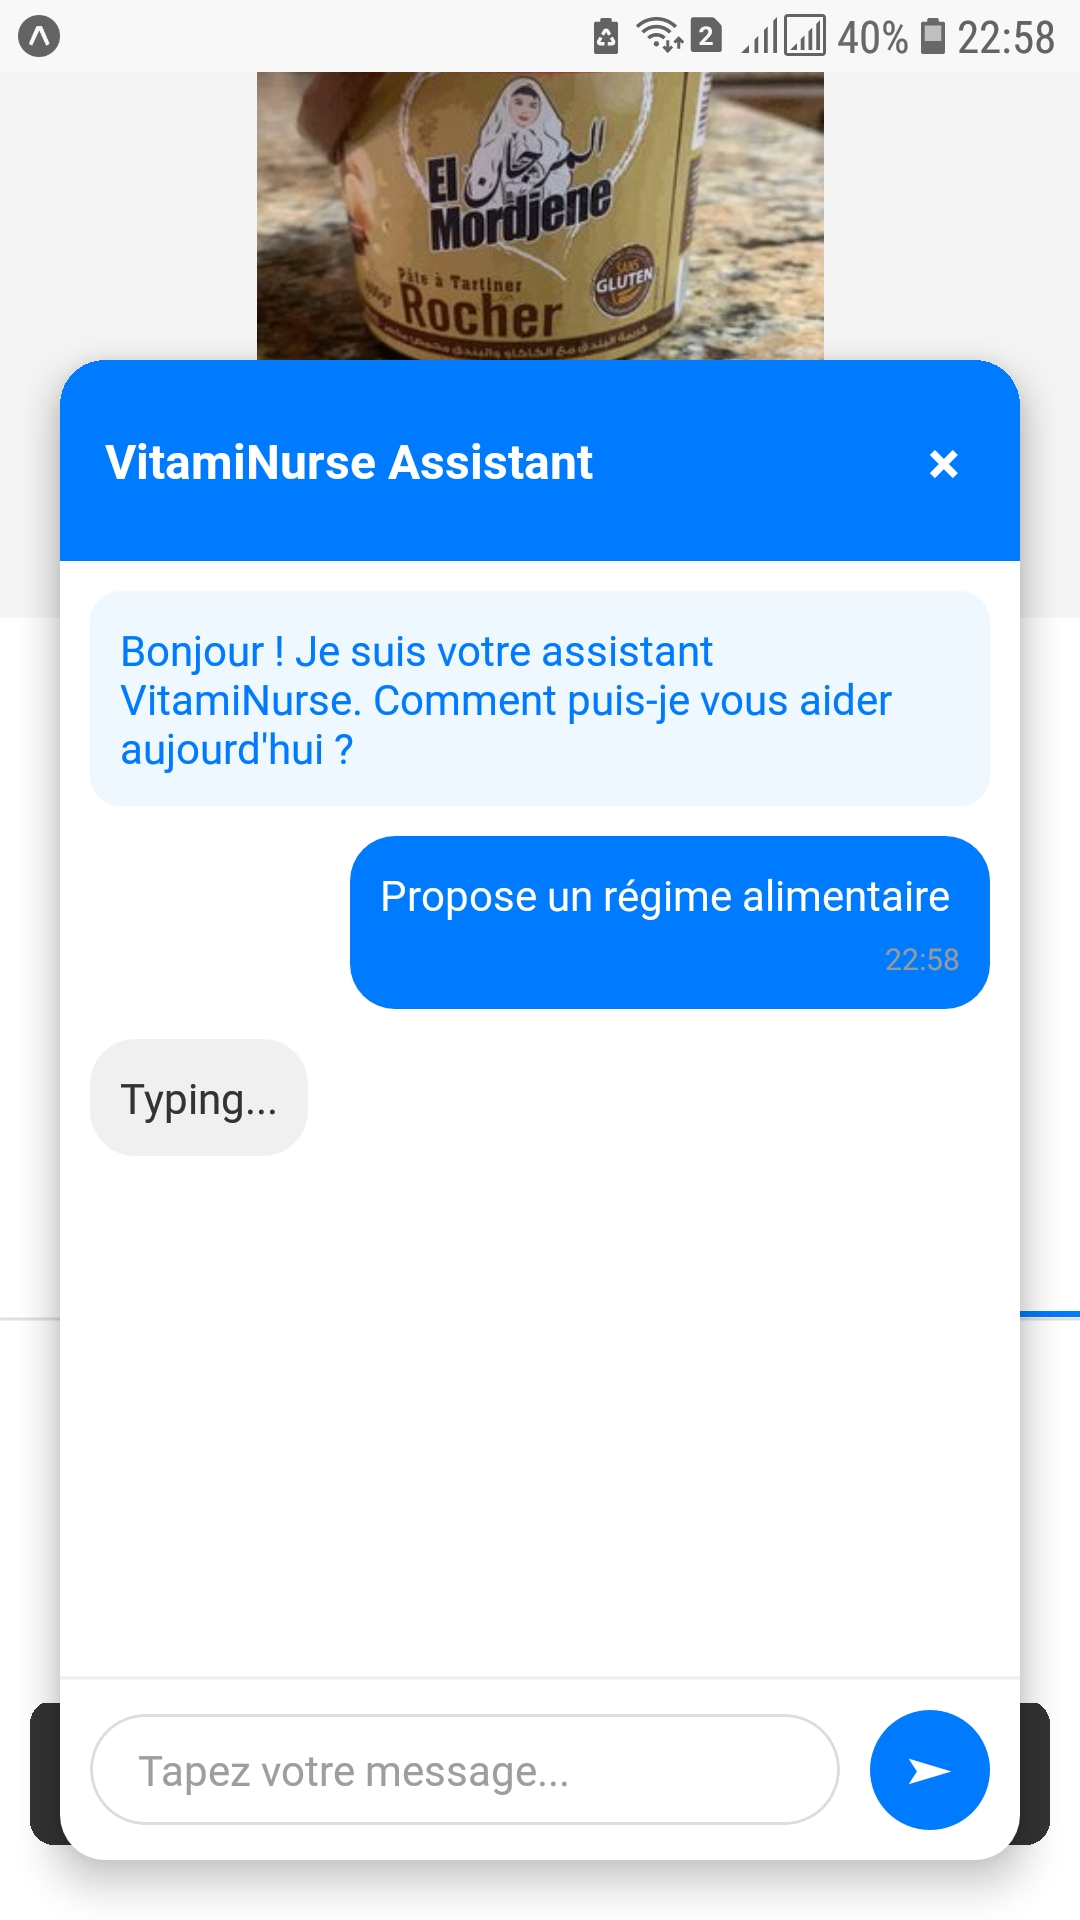
\includegraphics[width=0.51\textwidth]{images/chat_interface.jpg}
\caption{AI assistant chat interface} 
\label{fig:chatbot_interface}
\end{figure}
\end{center}


\subsection{Backend (FastAPI Server)}
The backend, developed using the \textbf{FastAPI} framework, functions as the system’s control hub. It is responsible for orchestrating communication between the mobile interface, AI reasoning layer, and data storage modules. Upon receiving a request, the backend validates the input, retrieves relevant product data from the nutritional database, and enriches it with user-specific profile information. It then constructs a prompt to be sent to the large language model (LLM), ensuring that all relevant dietary constraints and health conditions are explicitly included. The backend also maintains user session management, conversation history storage, and security protocols for handling sensitive health-related information. Thanks to FastAPI’s asynchronous capabilities, the backend can handle concurrent user requests with minimal latency, which is crucial for providing real-time responses.
\begin{center}
\begin{figure}[H]
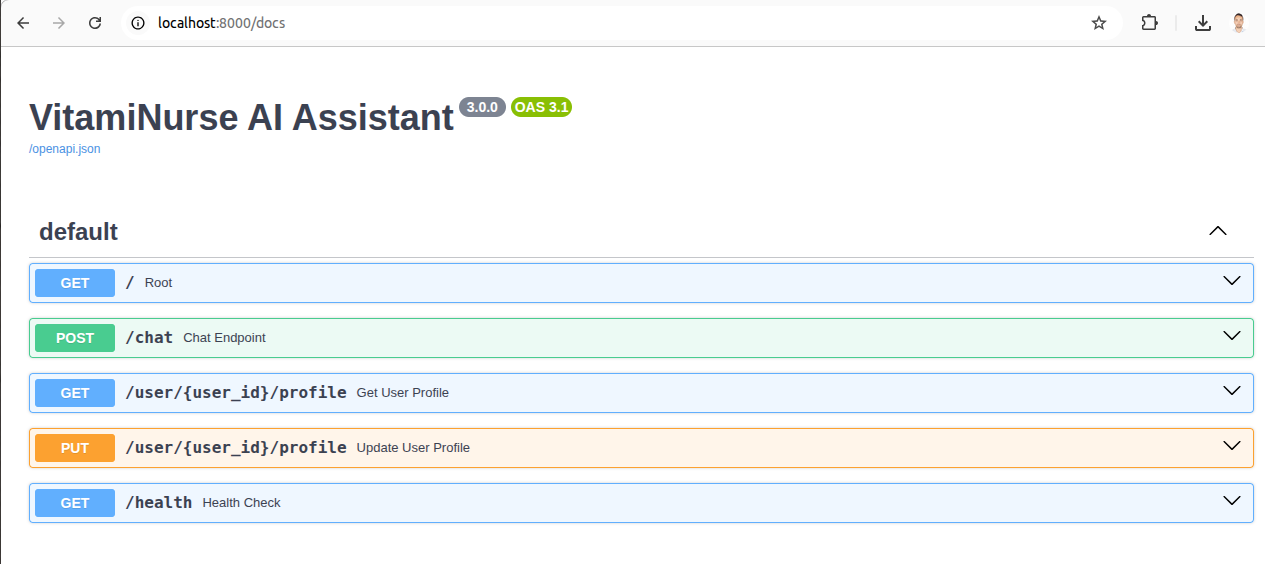
\includegraphics[width=0.9\textwidth]{images/chatbot_API.png}
\caption{Chatbot FastAPI} 
\label{fig:chatbot API}
\end{figure}
\end{center}

\subsection{AI and Data Layer}
The AI and data layer forms the intelligent core of the VitamiNurse assistant, leveraging advanced language models and sophisticated intent detection to deliver personalized nutritional guidance. At the heart of the system is OpenAI's \texttt{gpt-4o-mini} model, which is meticulously engineered through prompt crafting to provide structured, scientifically-grounded nutritional advice.

The system employs \texttt{LangChain} as its orchestration framework, enabling sophisticated intent detection and parallel processing of user requests. Through LangChain's structured output parsing with Pydantic models, the assistant can simultaneously handle multiple user intents including product searches, recipe generation, profile updates, and general nutritional inquiries.

A \texttt{ChromaDB} vector database serves as the persistent storage layer, maintaining semantic embeddings of user profiles, conversation history, and product information. This enables efficient retrieval and contextual understanding while ensuring data persistence across sessions.

The \emph{Recommendation Engine} introduced in the previous chapter is seamlessly integrated into this architecture. It operates on a hybrid approach combining collaborative filtering and content-based filtering, ensuring that recommended products are both personalized and nutritionally appropriate for each user's specific profile and constraints.


\section{Retrieval-Augmented Generation (RAG) in VitamiNurse}
\label{sec:rag}

\par Retrieval-Augmented Generation (RAG) is a hybrid architecture that enhances large language model (LLM) responses by dynamically retrieving relevant external knowledge and integrating it into the generation process \cite{lewis2020retrieval}. In the context of the \textit{VitamiNurse AI Assistant}, RAG enables personalized, context-aware nutritional guidance by retrieving user-specific health profiles and interaction history from a persistent vector database before generating responses. This approach ensures that advice is not only linguistically fluent but also grounded in the user’s unique physiological and dietary context. Formally, RAG decomposes into three sequential stages: Retrieval (R), Augmentation (A), and Generation (G) as illustrated in Figure~\ref{fig:RAG_architecture}

\begin{center}
\begin{figure}[H]
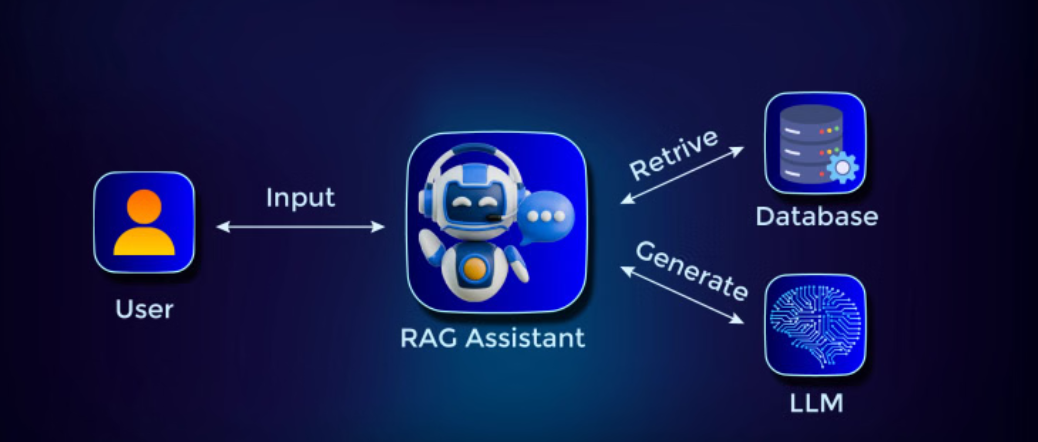
\includegraphics[width=0.98\textwidth]{images/RAG_logic.png}
\caption{RAG architecture in VitamiNurse} 
\label{fig:RAG_architecture}
\end{figure}
\end{center}

\subsection{Retrieval (R): User-Centric Context Fetching}
\label{subsec:retrieval}

The retrieval phase in VitamiNurse leverages \texttt{ChromaDB} to fetch semantically relevant user information. Specifically, two collections are maintained:
\begin{itemize}[label=-]
\item users : Stores structured user profiles (age, allergies, health conditions) as metadata, with embeddings generated via the \texttt{all-MiniLM-L6-v2} sentence transformer.
\item chat\_sessions : Archives past interactions to support short-term conversational memory.
\end{itemize}


When a user sends a message, the system retrieves their profile using their \texttt{user\_id}. This exact-match retrieval (by ID) is complemented by semantic capabilities for future extensions (e.g., similarity-based health cohort lookup). The retrieved profile serves as the primary source of personalization, aligning with RAG’s principle of grounding generation in external knowledge\cite{rag2020}.

\subsection{Augmentation (A): Dynamic Prompt Personalization}
\label{subsec:augmentation}

The augmentation phase constructs a system prompt that embeds the retrieved user profile into the LLM’s context window. VitamiNurse implements this via the \texttt{\_create\_personalized\_system\_prompt()} method, which formats user attributes (e.g., allergies, dietary preferences, pregnancy status) into natural language directives. For example:

\begin{quote}
    ``You are VitamiNurse, a nutrition AI. The user is a 32-year-old pregnant woman with celiac disease and a preference for high-fiber foods. Avoid gluten and prioritize iron-rich, pregnancy-safe options.''
\end{quote}

This step ensures the LLM’s internal reasoning is conditioned on factual, user-specific constraints—reducing hallucination risks and improving relevance. The augmented prompt, combined with recent conversation history (up to 6 turns), forms the complete input to the generator.

\subsection{Generation (G): Personalized Response Synthesis}
\label{subsec:generation}

The generation phase employs \texttt{gpt-4o-mini} model from OpenAI to produce concise and informed responses with specific instructions to limit replies to three sentences for clarity. In order to maintaining focus within the application’s intended scope ,the model is designed to gently but firmly redirect the discussion back to nutrition-related subjects.

\begin{quote}
    ``I can only provide nutritional advice. For medical concerns, please consult a healthcare professional.''
\end{quote}
Critically, generation it is \textit{conditioned} on the augmented prompt from the augmentation phase . After the response is sent, the conversation is saved in the background to the \textbf{chat sessions} database, and this closes the RAG loop by enabling future use of the interaction.

Additionally, the system uses the LLM itself to extract and update profile information from user messages such as detecting new allergies, effectively using generation to enrich the knowledge base this feature known as \textit{write-path RAG} }. In this case, the RAG system does not only retrieve and generate as in the traditional read-path process, but also updates or writes new information back into the user collection in ChromaDB based on chat interactions.

\section{Challenges and Solutions}
Throughout development, several significant challenges emerged in creating a robust conversational nutrition assistant. Maintaining coherent conversation context across extended interactions was addressed through LangChain's sophisticated memory management and ChromaDB's persistent conversation storage. Personalizing recommendations without burdening users with excessive input requirements was solved through GPT-4's intelligent information extraction capabilities, which automatically detect and update user profiles from natural conversation.

Ensuring structured, explainable nutritional advice was achieved through rigorous prompt engineering and Pydantic output parsing, enforcing consistent response formats. Handling ambiguous or incomplete user queries was resolved through the parallel intent processing architecture, which allows multiple interpretation paths to be explored simultaneously before synthesizing a comprehensive response.

The integration of multiple AI components (LangChain chains, GPT-4, ChromaDB, and the recommendation API) presented coordination challenges that were overcome through asynchronous processing patterns and robust error handling mechanisms.

\section{Future Improvements}
Planned enhancements focus on expanding the assistant's capabilities and integration points. Multi-modal support will enable image-based food recognition and nutritional analysis through advanced computer vision integration. Expanded wearable device connectivity will incorporate real-time physiological data from fitness trackers and health monitors, allowing for dynamic nutritional adjustments based on activity levels and metabolic states.

Advanced personalization through reinforcement learning will enable the system to continuously improve its recommendations based on user feedback and outcomes. Voice interaction capabilities will be enhanced through integration with popular voice assistants (Alexa, Google Assistant) and development of custom voice interfaces for hands-free nutritional guidance.

Additional planned features include:
\begin{itemize}
\item \textbf{Meal Planning Automation}: Multi-day meal planning with grocery list generation
\item \textbf{Social Features}: Community recipe sharing and nutritional challenges
\item \textbf{Healthcare Integration}: EHR connectivity for medical condition management
\item \textbf{Advanced Analytics}: Nutritional intake tracking and trend analysis
\end{itemize}


\section{Conclusion}
The VitamiNurse AI Nutrition Assistant represents a significant advancement in conversational healthcare applications by successfully integrating the Recommendation Engine into a sophisticated LangChain-powered architecture. The system demonstrates how parallel intent processing, dynamic profile management, and AI-generated content can create a comprehensive nutritional guidance platform.

By leveraging LangChain's orchestration capabilities alongside GPT-4's generative power and ChromaDB's persistent storage, VitamiNurse delivers personalized, context-aware dietary recommendations that adapt to users' evolving needs. The architecture successfully balances conversational flexibility with structured nutritional guidance, providing both immediate answers and long-term nutritional support.

This implementation positions VitamiNurse as a scalable foundation for digital health interventions, with the potential to expand into various healthcare domains beyond nutrition. The modular design ensures adaptability to new data sources, interaction modalities, and user requirements, making it well-suited for the evolving landscape of AI-powered healthcare applications.

The assistant not only provides immediate nutritional guidance but also serves as an educational tool, helping users develop sustainable healthy eating habits through personalized, explainable recommendations that consider their unique circumstances, preferences, and goals.

